% LaTeX .tex
% Example for the proceedings of the  25th International Congress of Mechanical Engineering
% COBEM 2019
% October, 20-25, 2019, Uberlândia, MG, Brazil
% Based on the template of the proceedings of COBEM2015 and COBEM2017

\documentclass[10pt,fleqn,a4paper,twoside]{article}
\usepackage{abcm}
\def\shortauthor{F. Author, S. Author and T. Author (update this heading accordingly)}
\def\shorttitle{Paper Short Title (First Letters Uppercase, make sure it fits in one line)}
\usepackage{subcaption}
\captionsetup{compatibility=false}
\usepackage{blindtext}
\begin{document}
\fphead
\hspace*{-2.5mm}\begin{tabular}{||p{\textwidth}}
\begin{center}
\vspace{-4mm}
\title{The mechanical properties of parts fabricated with PETG via fused deposition modeling}
\end{center}
\authors{Maíra Fernanda Oliveira de Miranda} \\
\authors{Felipe Jose Oliveira Ribeiro} \\
\authors{Alexandre Zuquete Guarato}\\
\institution{Federal University of Uberlândia (UFU), Av. João Naves de Ávila, 2121, Campos Santa Mônica, Uberlândia, MG } \\
\institution{mairaf\_miranda@hotmail.com} \\
\institution{feliperibeiro.ufu@gmail.com} \\
\institution{azguarato@ufu.br} \\
\\
\abstract{\textbf{Abstract.}  In the present paper, the authors aim to study the mechanical properties of parts made with the fusion deposition modeling process. Test specimens were made solid, with 100\% of infill, varying the extrusion temperature of the printed parts. Tensile tests were performed in each one of the twenty five test parts, being five for each extrusion temperature. It was studied the extrusion temperatures of: $230^\circ$, $235^\circ$, $240^\circ$, $245^\circ$ and $250^\circ$.It was observed that the (***** termianr com resultados)}\\
\\
\keywords{\textbf{Keywords:} FDM(Fused Deposition Modeling), PETG(Polyethylene Terephthalate Glycol), Young modulus, Poisson coefficient}\\
\end{tabular}

\section{INTRODUCTION}

PETG (Polyethylene Terephthalate Glycol) is a polymer that has been steadily gaining popularity among the 3D printing community, since it combines the reliability of PLA with the durability of ABS, the two most commonly used materials for FDM (Fused Deposition Modeling) \citep{tiposfilamento}. Such fact makes this polymer a good choice when prototyping mechanical parts. PETG may be considered better due to its increased strength, temperature and impact resistance when compared to PLA and ABS.

For all of its advantages, though, when it comes to the finished printed parts, its mechanical properties (as with others materials) present some complications \citep{3Dcomplication}. Since 3D printing is not yet well standardized by the manufacturers, it is impossible to safely predict the final properties of the parts by filament qualities. This problem becomes worse when considering the many parameters that influence the printing part of the process, such as printing temperature, rate, geometry and nozzle width. Another difficulty is that the final FDM part also becomes anisotropic \citep{PETG}, further complicating structural analysis. 

On the present paper, the authors aim to create a database of the mechanical properties of 3D printed parts made with the Prusa i3 MK2S Printer and out of PETG XT filament from 3Dfila. For that, several parameterizations of printing temperature and geometry were used to create testing parts with were subjected to tensile stress until rupture. From those tests the young modulus and Poisson coefficients were measured and used to formulate an statistical theoretical model. It is important to mention that these properties were chosen because they are needed to characterize the material on simulation softwares such as Ansys and Nastran for future structural analysis and material applications.  



\section{METHODOLOGY}

First it was made the specimens geometry for the study, as determined on the standard. After that, the parts were manufactured five at a time to increase uniformity. Then they were performed in the tensile test machine. The results were then treated statistically resulting in the mechanical properties for each temperature.


\vspace{3cm}


\section{SPECIMENS}

The tensile stress testing parts were designed following the geometry specified in the ASTM D638-02a standard (Type I specimen, with 7mm thickness) as utilized on \citep{test_on_fdm}. The geometry designed can be seen on Fig.\ref{fig1}:

\begin{figure*}[h!]
	\centering
	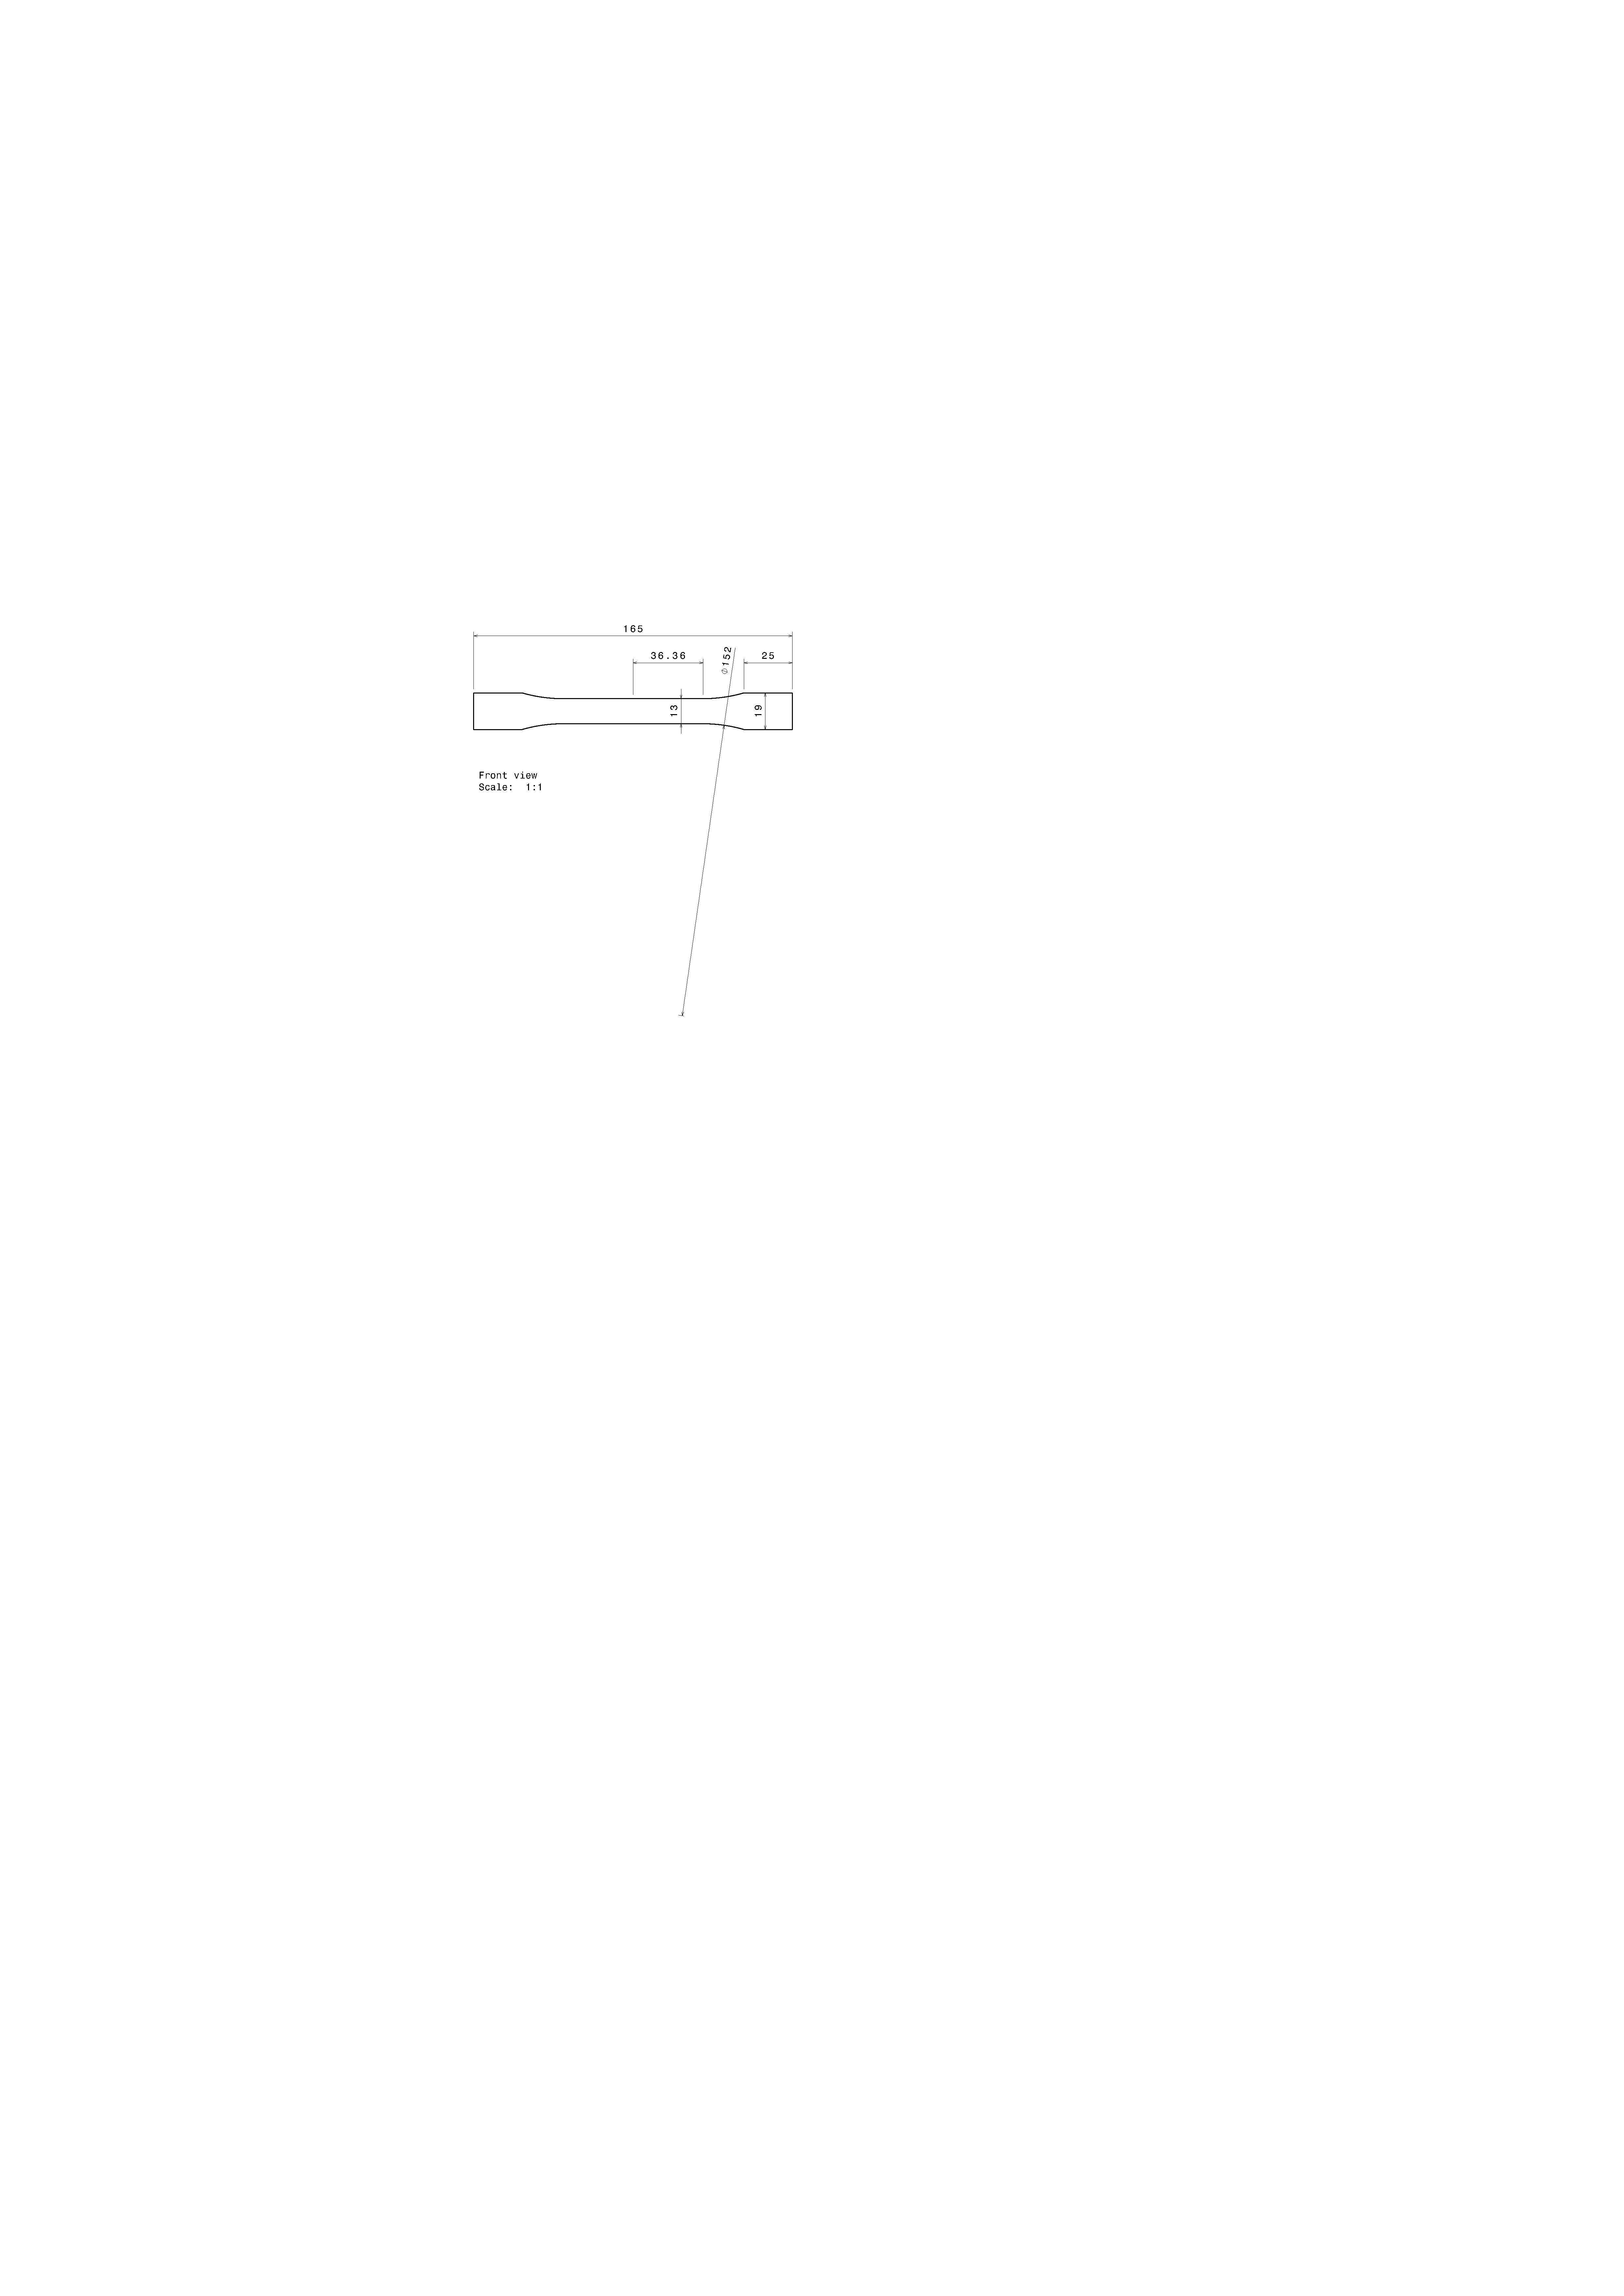
\includegraphics[ trim = {24cm 80cm 43cm 32cm}, clip , angle=0, scale=0.60 ]{imagens/Drawing1}
	\caption{Test parts CAD Draw.}
	\label{fig1}
\end{figure*}


From this scetch, a 3D model was created on a CAD software for printing (Figure \ref{fig2}). Such model was then exported as a STL file to the slicing software (Simplify3D), as seen on Fig.\ref{fig3}: 


\begin{figure*}[h!]
	\centering
	\begin{subfigure}[b]{0.5\textwidth}
		\centering
		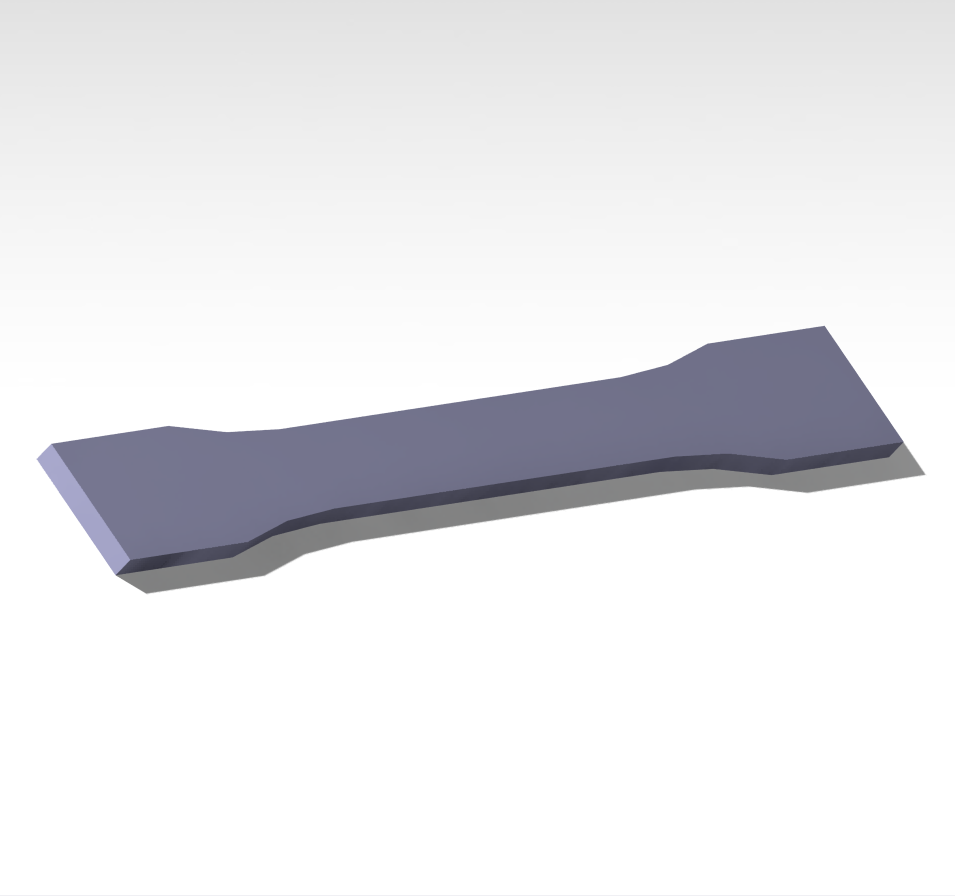
\includegraphics[ trim = {0 0 0 0}, clip , angle=0, scale=0.063 ]{imagens/renderizacao}
		\caption{CAD rendering.}
		\label{fig2}
	\end{subfigure}%
	~ 
	\begin{subfigure}[b]{0.5\textwidth}
		\centering
		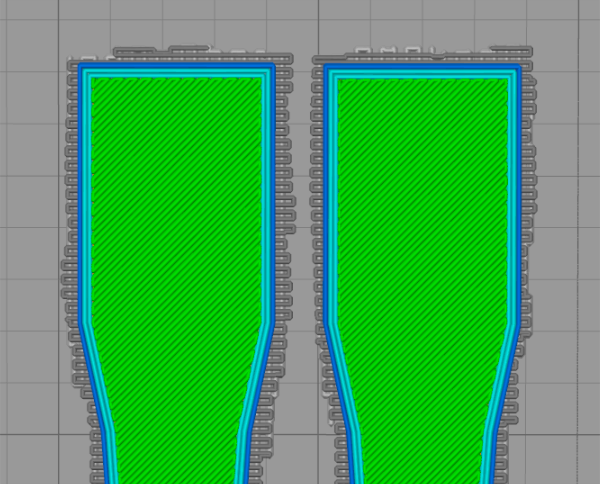
\includegraphics[ trim = {0cm 0cm 0 0cm}, clip , angle=0, scale=0.45 ]{imagens/Esboco2}
		\caption{Sliced part`s G code, made with Simplify3D software.}
		\label{fig3}
	\end{subfigure}
	\caption{Modeling and slicing of the specimen for printing.}
\end{figure*}

In the Figure \ref{fig3}, is possible to see that the parts were made on a support bed, in other words, not directly on the heated bed. Such method is used to secure the z axis regularity on the printed parts, as the fist layer printed directly over the heated plate has very different properties from the rest of the print \citep{PETG}. 

Is important to point here the qualities that will be set constantly throw all the test specimens. These parameters will not be discussed on the present paper: The Nozzle diameter was 0.4 mm, the retraction distance and speed were 5 mm and 2100 mm/min, the layer hight was 0.15 mm, with 3 lateral outer layers (Fig.\ref{fig3}) and the Heated bed were set to 80 degrees celsius.

The infill percentage was set to 100\%. The layers were made out of parallel lines and from one layer to the other the inclination of these lines varied $90^\circ$ from one another and made $45^\circ$ with the y axis of the print.









%
%\begin{table}[!h]
%\centering
%\caption{Experimental results for flexural properties of CFRC-4HS and CFRC-TWILL composites. \protect\\Span/depth ratio = 35:1. Average results of 7 specimens.}
%\begin{tabular}{|c|c|c|}
%\hline
%Composite Properties & CFRC-TWILL & CFRC-4HS\\
%\hline
%Flexural Strength (MPa)$^{(1)}$ & 209$\pm$ 10 & 180 $\pm$  15\\
%\hline
%Flexural Modulus (GPa)$^{(1)}$ & 57.0 $\pm$ 2.8 & 18.0 $\pm$  1.3\\
%\hline
%Mid-span deflection at the failure stress (mm) & 2.15 $\pm$  1.90 & 6.40 $\pm$  0.25\\
%\hline
%\end{tabular}
%\\
%\begin{tabular}{p{11cm}ll}
%$^{(1)}$ measured at 25$^{o}$C & &
%\end{tabular}
%\label{tab1}
%\end{table}






\section{MATERIAL PROCEDURES}
There was 25 test specimens, being 5 of each temperature. 


\section{PRELIMINARY RESULTS}
After the tests, all the data were taken and processed. Firs, these were the brute numerical result:

\begin{figure*}[h!]
	\centering
	\begin{subfigure}[b]{0.5\textwidth}
		\centering
		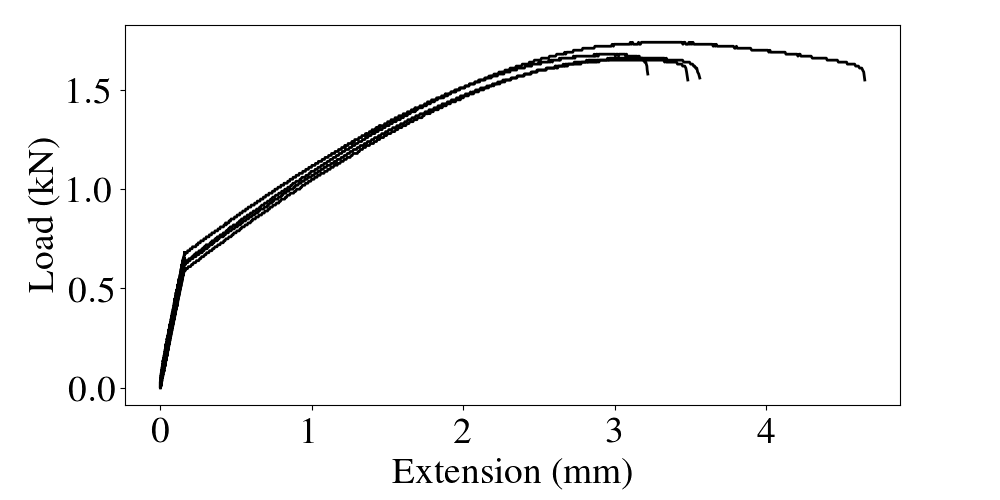
\includegraphics[ trim = {0 0 0 0}, clip , angle=0, scale=0.35 ]{imagens/230_bruto}
		\caption{For the temperature of $230^\circ$.}
		\label{fig2}
	\end{subfigure}%
	~ 
	\begin{subfigure}[b]{0.5\textwidth}
		\centering
		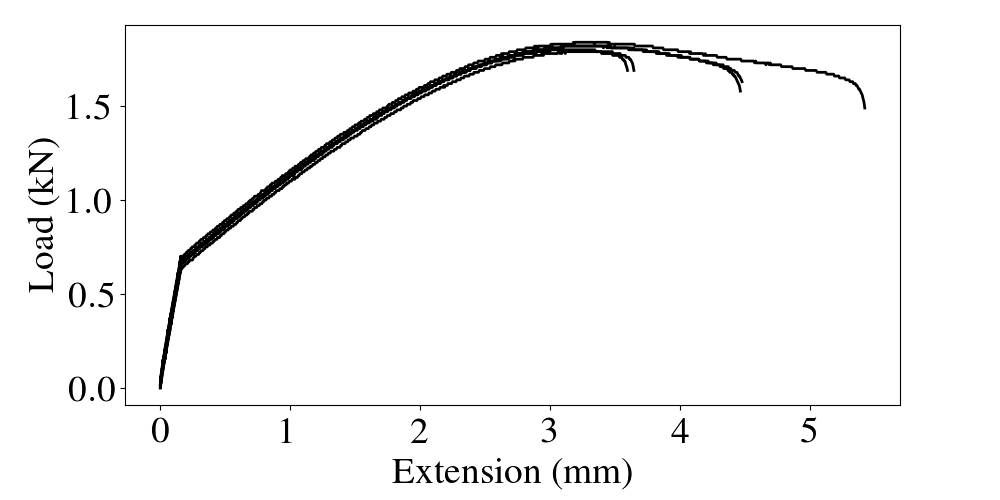
\includegraphics[ trim = {0cm 0cm 0 0cm}, clip , angle=0, scale=0.35 ]{imagens/235_bruto}
		\caption{For the temperature of $235^\circ$.}
		\label{fig3}
	\end{subfigure}
	\begin{subfigure}[b]{0.5\textwidth}
		\centering
		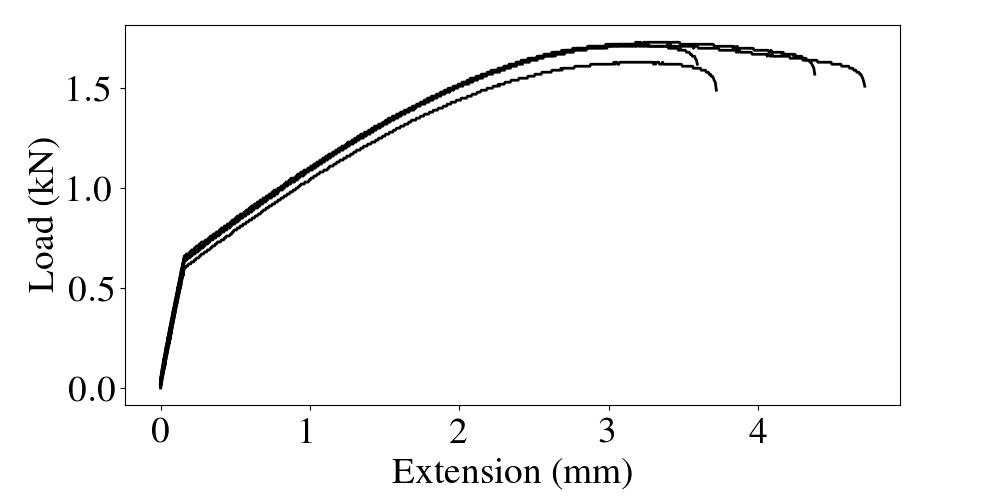
\includegraphics[ trim = {0 0 0 0}, clip , angle=0, scale=0.35 ]{imagens/240_bruto}
		\caption{For the temperature of $240^\circ$.}
		\label{fig4}
	\end{subfigure}%
	~ 
	\begin{subfigure}[b]{0.5\textwidth}
		\centering
		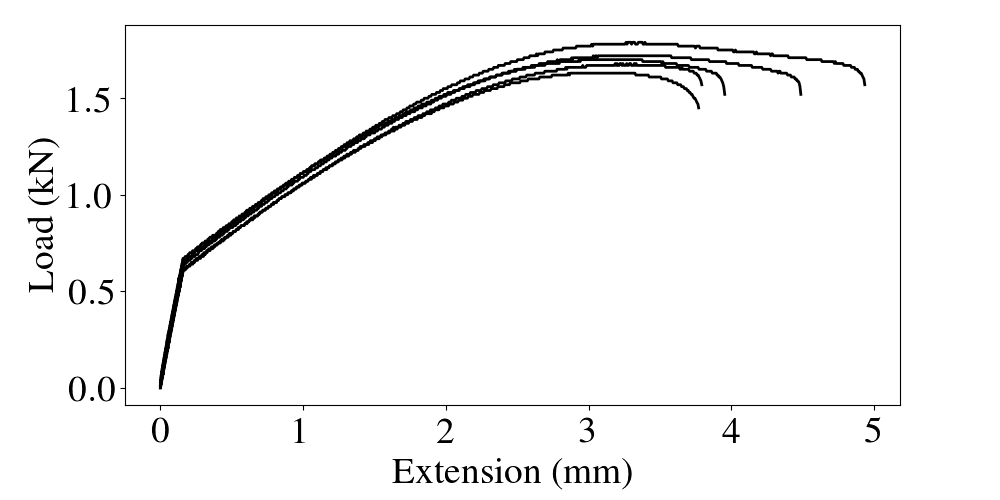
\includegraphics[ trim = {0cm 0cm 0 0cm}, clip , angle=0, scale=0.35 ]{imagens/245_bruto}
		\caption{For the temperature of $245^\circ$.}
		\label{fig5}
	\end{subfigure}
	\begin{subfigure}[b]{0.5\textwidth}
		\centering
		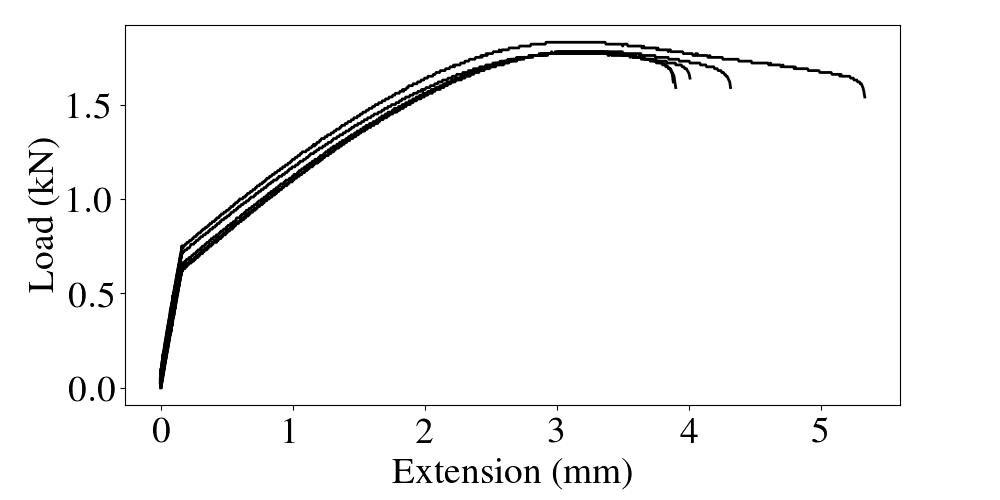
\includegraphics[ trim = {0cm 0cm 0 0cm}, clip , angle=0, scale=0.35 ]{imagens/250_bruto}
		\caption{For the temperature of $250^\circ$.}
		\label{fig6}
	\end{subfigure}

	\caption{Tensile tests performed on each specimen.}
\end{figure*}
 





\section{ACKNOWLEDGEMENTS}
The authors would like to thank the following professors and institutions: Dr. Ruham Pablo Reis, Dr. Pedro Pio Rosa Nishida, Lmest (Structural Mechanics Laboratory), FEMEC (Mechanical engineering College), UFU (Federal University of Uberl\^andia) and, especially, EPTA(Propulsion and Aerospace Technology Team) for financial support.




\section{REFERENCES} 

\bibliographystyle{abcm}
\renewcommand{\refname}{}
\bibliography{bibfile}

\end{document}
